% ****** Start of file apssamp.tex ******
%
%   This file is part of the APS files in the REVTeX 4 distribution.
%   Version 4.0 of REVTeX, August 2001
%
%   Copyright (c) 2001 The American Physical Society.
%
%   See the REVTeX 4 README file for restrictions and more information.
%
% TeX'ing this file requires that you have AMS-LaTeX 2.0 installed
% as well as the rest of the prerequisites for REVTeX 4.0
%
% See the REVTeX 4 README file
% It also requires running BibTeX. The commands are as follows:
%
%  1)  latex apssamp.tex
%  2)  bibtex prb
%  3)  latex apssamp.tex
%  4)  latex apssamp.tex
%
%\documentclass[aps,prb,preprint,groupedaddress,showpacs]{revtex4-1}
\documentclass[aps,prl,preprint,superscriptaddress]{revtex4}
%\documentclass[aps,prl,twocolumn,superscriptaddress]{revtex4}
%\documentclass[aps,prl,twocolumn,superscriptaddress]{revtex4}
%\documentclass[aps,prb,twocolumn,groupedaddress]{revtex4-1}


%\documentclass[twocolumn,showpacs,preprintnumbers,amsmath,amssymb]{revtex4}
%\documentclass[preprint,showpacs,preprintnumbers,amsmath,amssymb]{revtex4}

% Some other (several out of many) possibilities
%\documentclass[preprint,aps]{revtex4}
%\documentclass[preprint,aps,draft]{revtex4}
%\documentclass[prb]{revtex4}% Physical Review B

\usepackage{graphics}
\usepackage{graphicx}% Include figure files
\usepackage{epstopdf}
\usepackage{dcolumn}% Align table columns on decimal point
\usepackage{bm}% bold math
\usepackage{amsmath}
\usepackage{amssymb}
\usepackage{latexsym}
\usepackage{epsfig}
\usepackage{amsbsy}
\usepackage{array}
\usepackage{amssymb}
\usepackage{setspace}
\usepackage{bm}
\usepackage{float}

\newcommand{\ssint}{ - \!\!\!\!\! \int }
\def\sint{\ifmmode{- \!\!\!\!\!\! \int}
    \else{\hbox{$- \!\!\!\! \int \ $}}\fi}


\newcommand{\bsigma}{\boldsymbol{\sigma}}
\newcommand{\bmu}{\boldsymbol{\mu}}
\newcommand{\bvepsilon}{\boldsymbol{\varepsilon}}
\newcommand{\bepsilon}{\boldsymbol{\epsilon}}
\newcommand{\balpha}{\boldsymbol{\alpha}}
\newcommand{\bkappa}{\boldsymbol{\kappa}}
\newcommand{\bchi}{\boldsymbol{\chi}}
\newcommand{\bgamma}{\boldsymbol{\gamma}}
\newcommand{\bpsi}{\boldsymbol{\psi}}
\newcommand{\bnu}{\boldsymbol{\nu}}
\newcommand{\bzero}{\boldsymbol{0}}
\newcommand{\bbeta}{\boldsymbol{\beta}}
\newcommand{\bSigma}{\boldsymbol{\Sigma}}

\newcommand{\va}{\varphi}
\newcommand{\ep}{\epsilon}
\newcommand{\mbf}{{\bf m}}
\newcommand{\pbf}{{\bf p}}
\newcommand{\xbf}{{\bf x}}
\newcommand{\weak}{\rightharpoonup}
\newcommand{\rgoto}{\rightarrow}

\newcommand{\grad}{\mbox{grad}}
\newcommand{\curl}{\mbox{curl}}
\newcommand{\dive}{\mbox{div}}


\newcommand{\tr}{\mbox{tr}}

\newcommand{\ba}{\mathbf{a}}
\newcommand{\bb}{\mathbf{b}}
\newcommand{\bc}{\mathbf{c}}
\newcommand{\bd}{\mathbf{d}}
\newcommand{\be}{\mathbf{e}}
\newcommand{\bsf}{\mathbf{f}}
\newcommand{\bg}{\mathbf{g}}
\newcommand{\bsi}{\mathbf{i}}
\newcommand{\bk}{\mathbf{k}}
\newcommand{\bn}{\mathbf{n}}
\newcommand{\bo}{\mathbf{o}}
\newcommand{\bp}{\mathbf{p}}
\newcommand{\bq}{\mathbf{q}}
\newcommand{\br}{\mathbf{r}}
\newcommand{\bs}{\mathbf{s}}
\newcommand{\bt}{\mathbf{t}}
\newcommand{\bu}{\mathbf{u}}
\newcommand{\bv}{\mathbf{v}}
\newcommand{\bw}{\mathbf{w}}
\newcommand{\bx}{\mathbf{x}}
\newcommand{\by}{\mathbf{y}}
\newcommand{\bz}{\mathbf{z}}

\newcommand{\bca}{\mathbf{A}}
\newcommand{\bcb}{\mathbf{B}}
\newcommand{\bcc}{\mathbf{C}}
\newcommand{\bcd}{\mathbf{D}}
\newcommand{\bce}{\mathbf{E}}
\newcommand{\bcf}{\mathbf{F}}
\newcommand{\bcg}{\mathbf{G}}
\newcommand{\bch}{\mathbf{H}}
\newcommand{\bck}{\mathbf{K}}
\newcommand{\bcj}{\mathbf{J}}
\newcommand{\bci}{\mathbf{I}}
\newcommand{\bcl}{\mathbf{L}}
\newcommand{\bcm}{\mathbf{M}}
\newcommand{\bcn}{\mathbf{N}}
\newcommand{\bco}{\mathbf{O}}
\newcommand{\bcp}{\mathbf{P}}
\newcommand{\bcq}{\mathbf{Q}}
\newcommand{\bcr}{\mathbf{R}}
\newcommand{\bcs}{\mathbf{S}}
\newcommand{\bct}{\mathbf{T}}
\newcommand{\bcu}{\mathbf{U}}
\newcommand{\bcv}{\mathbf{V}}
\newcommand{\bcw}{\mathbf{W}}
\newcommand{\bcx}{\mathbf{X}}
\newcommand{\bcz}{\mathbf{Z}}
\newcommand{\bcy}{\mathbf{Y}}

%\nofiles

\begin{document}
	
	
	\title{Random Walk, Diffusion and Cluster Growth}% Force line breaks with \\
	
	\author{Xinyu Wu, Peifan Liu, Connor Hann and Xiaomeng Jia}
	\affiliation{Physics Department, Duke University}
	
	
	\date{\today}
	
	\begin{abstract}
		In this article,  
	\end{abstract}
	
	\maketitle
	
	\section{Introduction}  %This should be cancelled for PRL and APL. 
	
	
	
	\section{1. 2D Random Walk} 
	
	
	A random walk is a mathematical formalization of a path that consists of a succession of random steps. For one dimensional case, a random walker can move one step in $\pm x$ directions with equal probability at each time step. If we make consider the statistical properties of  an ensemble of random walkers, the expected value of the position $ <x> $ is zero, since the expectation of each step is zero. However, the root-mean-squared distance(RMS) after n steps is:
	
	\begin{equation}
	\sqrt{<x_n^2>} = \sqrt{\sum\limits_{i=1}^{n}\sum\limits_{j=1}^{n}<\Delta x_i\Delta x_j>} = \sqrt{n}\Delta x
	\end{equation} 
	Here $\Delta x$ is the step unit corresponding to a time unit $\Delta t$ and a constant velocity $v$:
	\begin{equation}
	\Delta x = v\cdot \Delta t
	\end{equation} 
	Combined with
	\begin{equation}
	n = \frac{t}{\Delta t}
	\end{equation}
	We can show that the motion is diffusive:
	\begin{equation}
	<x^2(t)> = 2Dt
	\end{equation}
	where $D = v\cdot\Delta x/2 = (\Delta x)^2/(2\Delta t)$ is the diffusion constant.
	
	If we generalize the deduction to the 2D case, where the random walkers can move one step in four diections ($\pm x, \pm y$) with equal probability, we can find that the motion is again diffusive, by evaluating the mean square distance:
	
	\begin{equation}
	<r^2(t)> = 2Dt
	\end{equation}
	Where $D = (\Delta x)^2/(4\Delta t)$.
	
	This argument can be verified numerically using Python. We write a program to simulate a random walker in 2 dimensions, taking steps
	of unit length in $\pm x$ or $\pm y$ direction on a discrete square lattice. For up to $n = 100$, by averaging over $10^4$ different walks for each $n > 3$, the expected value of the position $ <x> $ is zero at all time, and the mean square value  $ <x^2> $ has a linear relation with $n$(remember $n =t/\Delta t$ is proportional to $t$), as can be seen in Fig.1. A typical 2D random walking pattern is show in Fig.2. Since we choose $\Delta t = \Delta x = 1$ here, the diffusion constant is determined using the slope of $<r^2(t)>$ and $n$(see Fig.3):$D = 1/4$. 
	
		\begin{figure}[H]
			\centering
			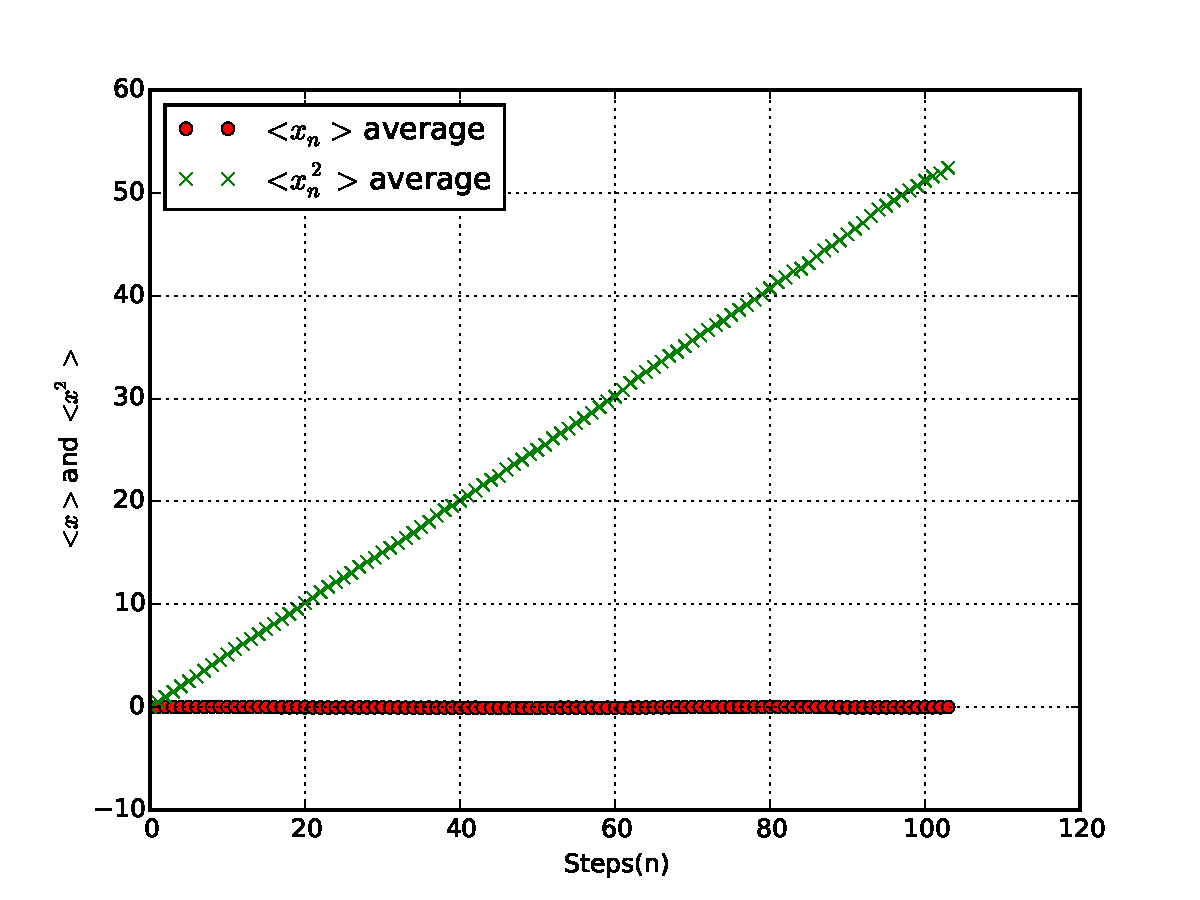
\includegraphics[width=1.0\textwidth]{rwxn.pdf}
			\caption{$ <x(t)> $ and  $ <x^2(t)> $ in 1D random walking, averaging over a 10000 random walker ensemble.}
		\end{figure}
			\begin{figure}[H]
				\centering
				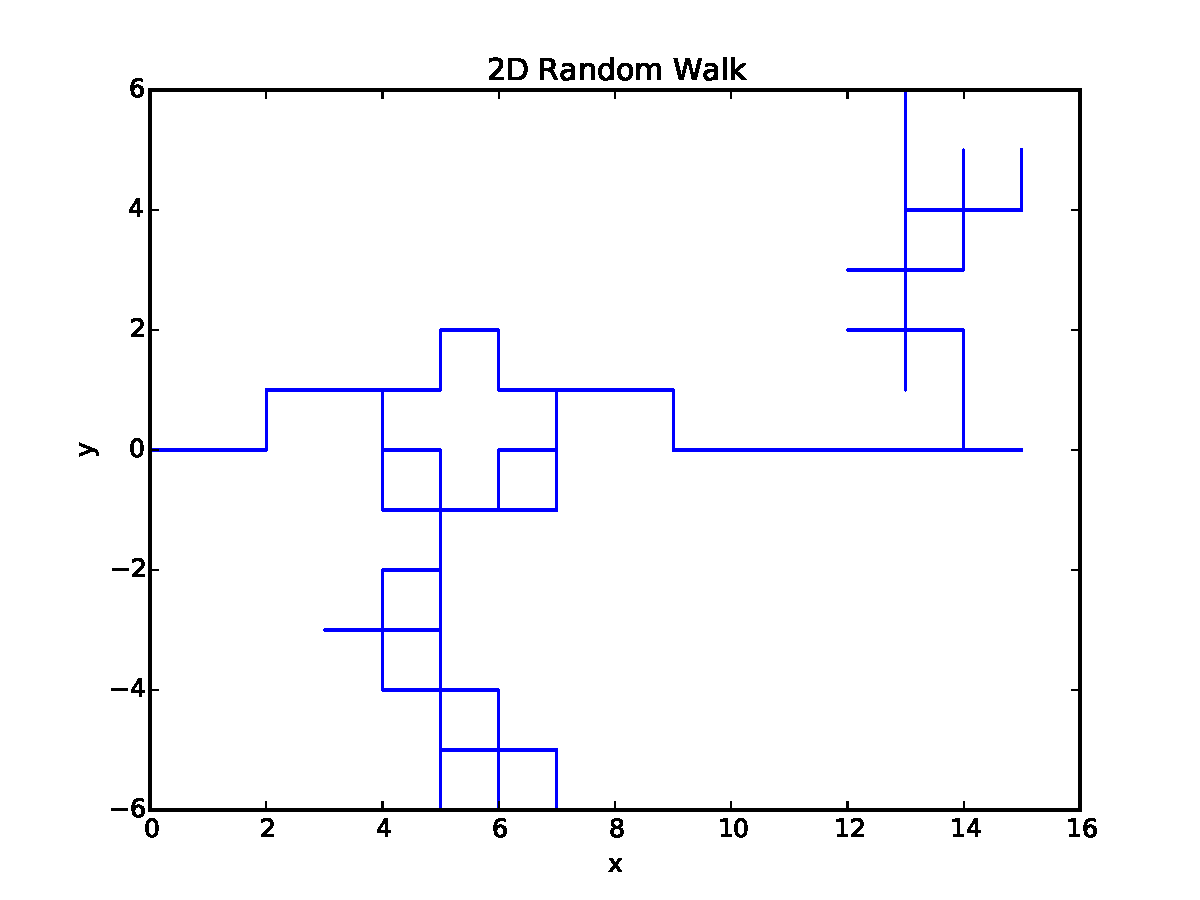
\includegraphics[width=1.0\textwidth]{rwxn3.pdf}
				\caption{A tipical 2D random walking pattern, starting from (0,0).}
			\end{figure}
		\begin{figure}[H]
			\centering
			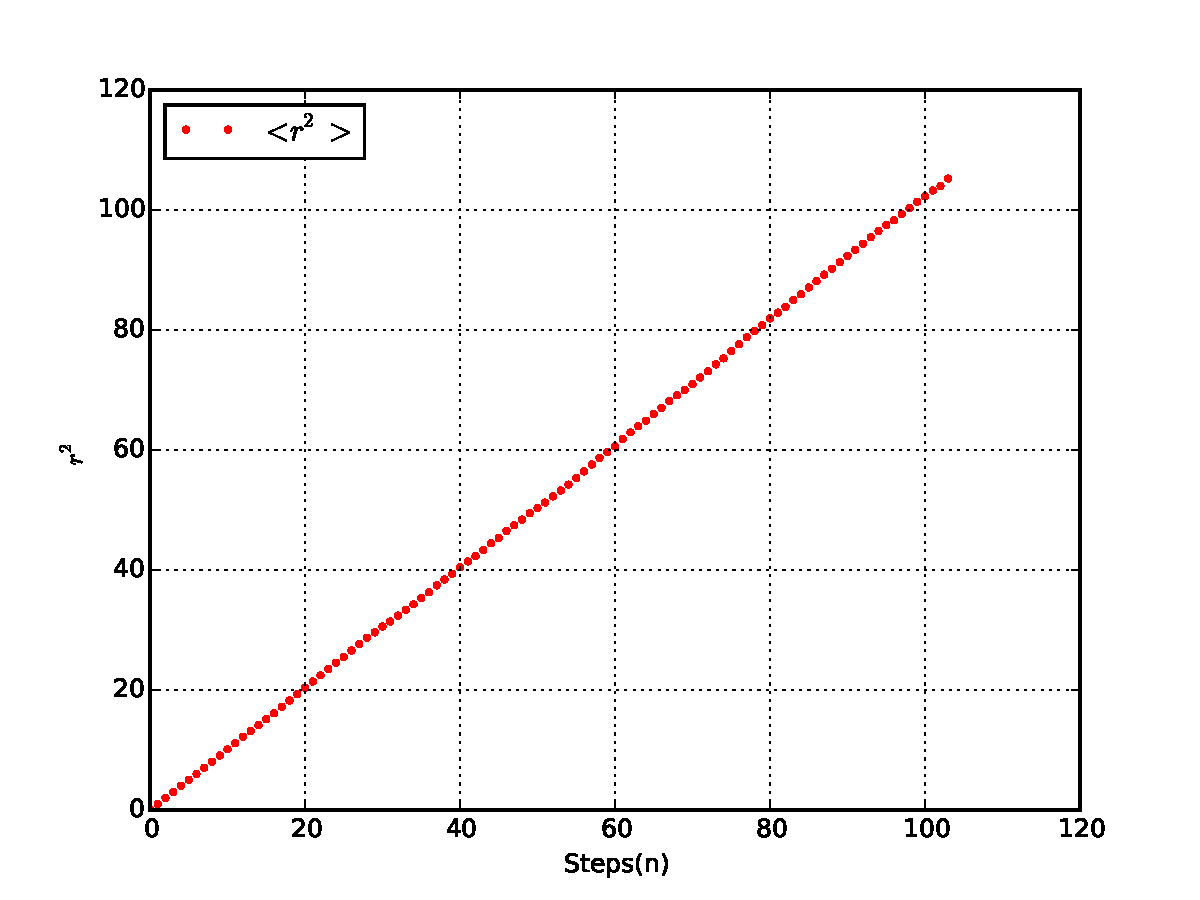
\includegraphics[width=1.0\textwidth]{rwxn2.pdf}
			\caption{$<r^2(t)>$ in 2D random walking, averaging over a 10000 random walker ensemble.}
		\end{figure}

	
	\section{2. Diffusion Equation}
	
	\section{3. Cluster Growth with the DLA model}

		%\begin{figure}[H]
		%	\centering
		%	\includegraphics[width=1.0\textwidth]{.eps}
		%	\caption{}
		%\end{figure}


	
\end{document}
	
	%
	% ****** End of file apssamp.tex ******
